\chapter{Monte Carlo Samples }\label{section:star_mc}
\ac{MC} samples used to correct data for detector effects were obtained by the embedding \ac{MC} technique~\cite{STAR:tpc}, in which  simulated particles are mixed with the real Zerobias events at the raw data level. Zerobias data events used in the embedding were sampled over the entire data-taking period in order to properly describe the data set used in the analysis.  Two samples of embedding MC were produced:
\begin{enumerate}
	\item Single particle \ac{MC}, in which particles are generated from flat distributions in $\eta$ and $p_\textrm{T}$, in order to have similar statistics in all bins.
	\item The \ac{SaS} model implemented in PYTHIA~8 with 4C tune. 
\end{enumerate}
The particles were propagated through the full simulation of the STAR TPC and RP system detectors using GEANT3~\cite{GEANT:three} and GEANT4~\cite{GEANT:four}, respectively. Obtained information for the simulated particles was embedded into the existing information of the real data. These events were next processed through the~full reconstruction chain. 

An~iterative unfolding procedure was used to express the track multiplicity in terms of the~number of charged particles.  The~unfolding matrices were obtained from PYTHIA~8 4C (\ac{SaS}). In order to keep statistical precision coming
from the~matrices high, samples filtered on true-level values of $\xi$ and $t$ (not necessarily with reconstructed proton track in RP) are used. 

It is preferred to get the detector corrections from a~MC, which is dedicated to simulate the~studied  physics process. However, for this purpose, the statistics in the MC should be several times greater than we have in the data for analysis. Since this is not possible with  low efficiency of TPC and TOF, the basic method of corrections used in the analysis for $p_\textrm{T}$ and $\bar{\eta}$ distributions is a~method of factorization of global efficiency into the product of single-particle efficiencies. In this way, statistically precise multidimensional corrections on TPC and TOF were obtained from the~single particle MC. %These corrections were not applied to charged-particle multiplicity distributions since  the~unfolding matrices already contain TPC and TOF efficiencies.
The~charged-particle multiplicity distributions were unfolded from the~measured multiplicities of TPC tracks based on the~response matrix, which takes into account  all detector effects and was obtained from PYTHIA 8 4C (SaS) simulation of SD process. In this procedure single particle MC samples were not used.  



%For charged-particle multiplicity distributions 
 %Dla n_ch  robi Pan unfolding i korzysta z PYTHII.
 %To trzeba napisać.  Ale nadal  jak rozumiem faktoryzuje Pan stan centralny i protony do przodu w tym sensie, że macierze odpowiedzi maja cięcie na 
 %xi i t na poziomie true, bez wymagania obserwacji protonu w RP.

Several additional MC samples were generated, in which  simulated particles were propagated through full simulation and reconstruction chain but were  not embedded  into Zerobias events.   
Systematic effect related to hadronization of the diffractive system was determined by using an~alternative hadronization model implemented in HERWIG. Results are compared to model predictions from PYTHIA 8 4C (\ac{SaS}), HERWIG, EPOS and alternative PYTHIA 8 model  \ac{MBR}  with A2 tune. EPOS predicts very large contribution of forward 
protons, which originate from non-diffractive events and are well separated in rapidity from other final state particles. This is the result of low mass excitation of the proton remnant ($<1$ GeV) leading to hadronization of the beam remnant back to the proton. Therefore EPOS predictions were separated in two classes: diffractive (EPOS SD) modelled by Pomeron exchange and non-diffractive modelled  by low mass excitation of the proton remnant (EPOS SD$^\prime$). Such remnant treatment is very unique in EPOS compared to other string models, especially, to that used in PYTHIA~8, where \ac{ND} forward protons are rare 
and  arise from string fragmentation and hadronization. In all PYTHIA~8 models, diffractive cross-sections are scaled by the~fudge factors, which were introduced in order to describe the~full phase space~\cite{Sjostrand:2006za,MBR:intro}. In the~\ac{SaS} model, the~fudge factors for SD and DD,  $F_{\textrm{SD}}$ and $F_{\textrm{DD}}$, are defined as a~function of diffractive masses:

\begin{equation}
F_{\textrm{SD}}=\left(1-\frac{M^2}{s}\right)\left(1+\frac{c_\textrm{res}M^2_\textrm{res}}{M^2_\textrm{res}+M^2}\right)
\end{equation}

\begin{equation}
F_{\textrm{DD}}=\left(1-\frac{M_a^2+M_b^2}{s}\right)\left(\frac{sm^2_p}{sm^2_p+M_a^2M_b^2}\right)\times
\left(1+\frac{c_\textrm{res}M_\textrm{res}^2}{M_\textrm{res}^2+M_a^2}\right)\left(1+\frac{c_\textrm{res}M_\textrm{res}^2}{M_\textrm{res}^2+M_b^2}\right)
\end{equation}
where $M$ and $M_{a}$, $M_{b}$ are the~invariant masses of the~systems $X$ and $X_a$, $X_b$ for SD and DD, respectively, $c_\textrm{res}=2$ and $M_\textrm{res}=2$~GeV/c$^2$ were obtained from a~fit to $pp/\bar{p}p$ data~\cite{Sjostrand:2006za}. On the~other hand, in the~\ac{MBR} model the~fudge factor is given as a function of the~rapidity gap~\cite{MBR:intro}:
\begin{equation}
S=\frac{1}{2}\left[1+\textrm{erf}\left(\frac{\Delta y-\Delta y_S}{\sigma_S}\right)\right]
\end{equation}
where $\Delta y$ is the~rapidity gap, $\Delta y_S=2$ and $\sigma_S=0.5$. As a result, diffractive cross sections are artificially suppressed at 
relatively large values of $\xi$ ($>$0.05). This artificial suppression significantly changes predicted distribution of $\xi$ and fractions of different processes in our fiducial phase space. Therefore data is also compared with expectations obtained without suppression of the~diffractive cross sections (MBR-tuned).

Figure~\ref{fig:STARtrueMC} shows $\xi$ and $|t|$ distributions generated with  EPOS (SD and SD+SD$^\prime$) and PYTHIA~8 SD (MBR and MBR-tuned). There are differences among models in both the~low and high $\xi$ regions. EPOS SD is only relevant for very small $|t|$ and is suppressed in the~STAR acceptance region, $0.04<|t|<0.16$, where EPOS SD$^\prime$ contribution dominates. In addition, the $t$-slope is  very different for EPOS SD and SD$^\prime$, while it is similar for EPOS SD$^\prime$ and PYTHIA~8 predictions. The~PYTHIA~8 (MBR-tuned) expectations, as opposed to the~MBR model,  lead
to the~larger cross-sections in the high-mass regions.
 
\begin{figure}[h!]
	\centering
	\includegraphics[width=0.49\textwidth, page=14]{chapters/dataSampleSTAR/img/true.pdf}
	\includegraphics[width=0.49\textwidth, page=13]{chapters/dataSampleSTAR/img/true.pdf}
	\caption{(left) $\xi$ and  (right) $|t|$ distributions for various MC generators at $\sqrt{s} = 200$~GeV.}
	\label{fig:STARtrueMC}
\end{figure}